%- - - - - - - - - - - - - - - - - - - - - - - - - - - - - - - - - ESTRUTURAS DE DADOS -
%- - - - - - - - - - - - - - - - - - - - - - - - - - - - - - - - - SLIDE -

% array static / vector ..
% problema / motivação
%    recuperar um valor de acordo com diferentes politicas
% 	 stack
% 	 queue
% 	 PQ
% C++ String
% BST -- set, map
% STL - sort, algorithm...


\begin{frame}
\frametitle{Estruturas de Dados Básicas}
\begin{block}{Objetivo}
Apresentar algumas estruturas de dados básicas e comumente usadas em competições.
\begin{itemize}
	\bitem Foco na aplicação das mesmas, utilizando a \emph{Standard Library} do C++.
\end{itemize}
\end{block}
\end{frame}

%- - - - - - - - - - - - - - - - - - - - - - - - - - - - - - - - - SLIDE -
\begin{frame}
\frametitle{Estruturas de Dados Básicas}
\begin{block}{Vetores}
\begin{itemize}
	\bitem Vetor estático -- \texttt{int array[256];}
	\bitem Vetor dinâmico 
	\begin{itemize}
		\bitem C++ \emph{Standard Library} \textbf{vector}, Java \textbf{Vector}
	\end{itemize}
\end{itemize}
\end{block}

\begin{block}{STL vector}
\begin{itemize}
	\item[] \texttt{\#include<vector>}
	\begin{itemize}
		\item[] \texttt{vector<int> a;    a.push\_back(x); }
		\item[] \texttt{vector<int> a(15);  a[10] = 42;}
		\item[] \texttt{vector<int> a(15, -1);}
		\item[] \texttt{vector<char> b; vector<double> c;}
		\item[] \texttt{vector<int> a; a.resize(1337); }
	\end{itemize}
\end{itemize}
\end{block}
\end{frame}

%- - - - - - - - - - - - - - - - - - - - - - - - - - - - - - - - - SLIDE -
\defverbatim[colored]\lstI{
\begin{lstlisting}[language=C++]
void semestre() {
	while(true) { /* nunca para */
		tarefa x = PegaNovaTarefa(tarefas);
		processa(x);
		/* novas tarefas podem surgir */
	}
}
\end{lstlisting}
}


\begin{frame}
\frametitle{Estruturas de Dados Básicas}
\begin{block}{Semestre típico}
\lstI
\end{block}

\begin{block}{}
	\begin{itemize}
		\bitem PegaNovaTarefa() decide a ordem em que as tarefas serão selecionadas.
	\end{itemize}
\end{block}

\end{frame}

%- - - - - - - - - - - - - - - - - - - - - - - - - - - - - - - - - SLIDE -
\begin{frame}
\frametitle{Estruturas de Dados Básicas}
\begin{block}{PegaNovaTarefa()}
\begin{itemize}
	\bitem Possíveis comportamentos de PegaNovaTarefa():
	\begin{itemize}
		\bitem Retorna a tarefa mais nova
		\bitem Retorna a tarefa mais velha
		\bitem Retorna a tarefa mais urgente
		\bitem Retorna a tarefa mais fácil
	\end{itemize}
	\bitem Queremos que PegaNovaTarefa() execute no menor tempo possível:
	\begin{itemize}
		\bitem ... organizando as tarefas de uma forma inteligente
	\end{itemize}
\end{itemize}
\end{block}
\end{frame}

%- - - - - - - - - - - - - - - - - - - - - - - - - - - - - - - - - SLIDE -
\begin{frame}
\frametitle{Estruturas de Dados Básicas}
\begin{block}{PegaNovaTarefa()}
\begin{itemize}
	\bitem Possíveis comportamentos de PegaNovaTarefa():
	\begin{itemize}
		\bitem Retorna a tarefa mais nova (pilha)
		\bitem Retorna a tarefa mais velha
		\bitem Retorna a tarefa mais urgente
		\bitem Retorna a tarefa mais fácil
	\end{itemize}
	\bitem Queremos que PegaNovaTarefa() execute no menor tempo possível:
	\begin{itemize}
		\bitem ... organizando as tarefas de uma forma inteligente
	\end{itemize}
\end{itemize}
\end{block}
\end{frame}

%- - - - - - - - - - - - - - - - - - - - - - - - - - - - - - - - - SLIDE -
\begin{frame}
\frametitle{Estruturas de Dados Básicas}
\begin{block}{Pilha}
\begin{itemize}
	\bitem Ultimo que entra é o primeiro que sai (LIFO)
	\bitem Suporta três operações de tempo constante:
	\begin{itemize}
		\bitem Push(x): Insere x na pilha
		\bitem Pop(): Remove o item mais novo
		\bitem Top(): Retorna o item mais novo
	\end{itemize}
	\bitem Implementação pronta na STL (stack)
\end{itemize}
\end{block}
\end{frame}

%- - - - - - - - - - - - - - - - - - - - - - - - - - - - - - - - - SLIDE -
\begin{frame}
\frametitle{Estruturas de Dados Básicas}
\begin{block}{STL - Stack}
\begin{itemize}
	\bitem empty() Testa se a pilha está vazia
	\begin{itemize}
		\bitem Complexidade - $O(1)$
	\end{itemize}
	\bitem size() Retorna o tamanho da pilha
	\begin{itemize}
		\bitem Complexidade - $O(1)$
	\end{itemize}
	\bitem top() Retorna o topo da pilha
	\begin{itemize}
		\bitem Complexidade - $O(1)$
	\end{itemize}
	\bitem push(elemento) Insere um elemento na pilha
	\begin{itemize}
		\bitem Complexidade - $O(1)$
	\end{itemize}
	\bitem pop() Retira um elemento da pilha
	\begin{itemize}
		\bitem Complexidade - $O(1)$
	\end{itemize}
\end{itemize}
\end{block}
\end{frame}

%- - - - - - - - - - - - - - - - - - - - - - - - - - - - - - - - - SLIDE -
\begin{frame}
\frametitle{Estruturas de Dados Básicas}
\begin{block}{PegaNovaTarefa()}
\begin{itemize}
	\bitem Possíveis comportamentos de PegaNovaTarefa():
	\begin{itemize}
		\bitem Retorna a tarefa mais nova (pilha)
		\bitem Retorna a tarefa mais velha
		\bitem Retorna a tarefa mais urgente
		\bitem Retorna a tarefa mais fácil
	\end{itemize}
	\bitem Queremos que PegaNovaTarefa() execute no menor tempo possível:
	\begin{itemize}
		\bitem ... organizando as tarefas de uma forma inteligente
	\end{itemize}
\end{itemize}
\end{block}
\end{frame}

%- - - - - - - - - - - - - - - - - - - - - - - - - - - - - - - - - SLIDE -
\begin{frame}
\frametitle{Estruturas de Dados Básicas}
\begin{block}{PegaNovaTarefa()}
\begin{itemize}
	\bitem Possíveis comportamentos de PegaNovaTarefa():
	\begin{itemize}
		\bitem Retorna a tarefa mais nova (pilha)
		\bitem Retorna a tarefa mais velha (fila)
		\bitem Retorna a tarefa mais urgente
		\bitem Retorna a tarefa mais fácil
	\end{itemize}
	\bitem Queremos que PegaNovaTarefa() execute no menor tempo possível:
	\begin{itemize}
		\bitem ... organizando as tarefas de uma forma inteligente
	\end{itemize}
\end{itemize}
\end{block}
\end{frame}

%- - - - - - - - - - - - - - - - - - - - - - - - - - - - - - - - - SLIDE -
\begin{frame}
\frametitle{Estruturas de Dados Básicas}
\begin{block}{Fila}
\begin{itemize}
	\bitem Primeiro que entra é o primeiro que sai (FIFO)
	\bitem Suporta três operações de tempo constante:
	\begin{itemize}
		\bitem Push(x): Insere x na fila
		\bitem Pop(): Remove o item mais velho
		\bitem Front(): Retorna o item mais velho
	\end{itemize}
	\bitem Implementação pronta na STL (queue)
\end{itemize}
\end{block}
\end{frame}

%- - - - - - - - - - - - - - - - - - - - - - - - - - - - - - - - - SLIDE -
\begin{frame}
\frametitle{Estruturas de Dados Básicas}
\begin{block}{STL - Queue}
\begin{itemize}
	\bitem empty() Testa se a fila está vazia
	\begin{itemize}
		\bitem Complexidade - $O(1)$
	\end{itemize}
	\bitem size() Retorna o tamanho da fila
	\begin{itemize}
		\bitem Complexidade - $O(1)$
	\end{itemize}
	\bitem front() Retorna quem está na frente da fila
	\begin{itemize}
		\bitem Complexidade - $O(1)$
	\end{itemize}
	\bitem back() Retorna quem está no fim da fila
	\begin{itemize}
		\bitem Complexidade - $O(1)$
	\end{itemize}
	\bitem push(elemento) Insere um elemento na fila
	\begin{itemize}
		\bitem Complexidade - $O(1)$
	\end{itemize}
	\bitem pop() Retira um elemento da fila
	\begin{itemize}
		\bitem Complexidade - $O(1)$
	\end{itemize}
\end{itemize}
\end{block}
\end{frame}

%- - - - - - - - - - - - - - - - - - - - - - - - - - - - - - - - - SLIDE -
\begin{frame}
\frametitle{Estruturas de Dados Básicas}
\begin{block}{PegaNovaTarefa()}
\begin{itemize}
	\bitem Possíveis comportamentos de PegaNovaTarefa():
	\begin{itemize}
		\bitem Retorna a tarefa mais nova (pilha)
		\bitem Retorna a tarefa mais velha (fila)
		\bitem Retorna a tarefa mais urgente
		\bitem Retorna a tarefa mais fácil
	\end{itemize}
	\bitem Queremos que PegaNovaTarefa() execute no menor tempo possível:
	\begin{itemize}
		\bitem ... organizando as tarefas de uma forma inteligente
	\end{itemize}
\end{itemize}
\end{block}
\end{frame}

%- - - - - - - - - - - - - - - - - - - - - - - - - - - - - - - - - SLIDE -
\begin{frame}
\frametitle{Estruturas de Dados Básicas}
\begin{block}{PegaNovaTarefa()}
\begin{itemize}
	\bitem Possíveis comportamentos de PegaNovaTarefa():
	\begin{itemize}
		\bitem Retorna a tarefa mais nova (pilha)
		\bitem Retorna a tarefa mais velha (fila)
		\bitem Retorna a tarefa mais urgente (fila de prioridades)
		\bitem Retorna a tarefa mais fácil
	\end{itemize}
	\bitem Queremos que PegaNovaTarefa() execute no menor tempo possível:
	\begin{itemize}
		\bitem ... organizando as tarefas de uma forma inteligente
	\end{itemize}
\end{itemize}
\end{block}
\end{frame}

%- - - - - - - - - - - - - - - - - - - - - - - - - - - - - - - - - SLIDE -
\begin{frame}
\frametitle{Estruturas de Dados Básicas}
\begin{block}{PegaNovaTarefa()}
\begin{itemize}
	\bitem Possíveis comportamentos de PegaNovaTarefa():
	\begin{itemize}
		\bitem Retorna a tarefa mais nova (pilha)
		\bitem Retorna a tarefa mais velha (fila)
		\bitem Retorna a tarefa mais urgente (fila de prioridades)
		\bitem Retorna a tarefa mais fácil (fila de prioridades)
	\end{itemize}
	\bitem Queremos que PegaNovaTarefa() execute no menor tempo possível:
	\begin{itemize}
		\bitem ... organizando as tarefas de uma forma inteligente
	\end{itemize}
\end{itemize}
\end{block}
\end{frame}

%- - - - - - - - - - - - - - - - - - - - - - - - - - - - - - - - - SLIDE -
\begin{frame}
\frametitle{Estruturas de Dados Básicas}
\begin{block}{Fila de prioridades}
\begin{itemize}
	\bitem Cada elemento em uma fila de prioridades tem um valor que corresponde a sua prioridade
	\bitem Suporta três operações
	\begin{itemize}
		\bitem Push(x, p): Insere x com prioridade p na fila de prioridades
		\bitem Pop(): Remove o elemento com a maior prioridade
		\bitem Top(): Retorna o elemento com a maior prioridade
	\end{itemize}
	\bitem Todas as operações podem ser feitas de forma rápida se implementadas usando uma Heap
	\bitem Implementação com Heap pronta na STL (priority\_queue)
\end{itemize}
\end{block}
\end{frame}

%- - - - - - - - - - - - - - - - - - - - - - - - - - - - - - - - - SLIDE -
\begin{frame}
\frametitle{Estruturas de Dados Básicas}
\begin{block}{STL - Priority Queue}
\begin{itemize}
	\bitem empty() Testa se a fila está vazia
	\begin{itemize}
		\bitem Complexidade - $O(1)$
	\end{itemize}
	\bitem size() Retorna o tamanho da fila
	\begin{itemize}
		\bitem Complexidade - $O(1)$
	\end{itemize}
	\bitem top() Retorna a frente da fila
	\begin{itemize}
		\bitem Complexidade - $O(1)$
	\end{itemize}
	\bitem push(element) Insere um elemento na fila
	\begin{itemize}
		\bitem Complexidade - $O(log\ n)$
	\end{itemize}
	\bitem pop() Retira um elemento da fila
	\begin{itemize}
		\bitem Complexidade - $O(log\ n)$
	\end{itemize}
\end{itemize}
\end{block}
\end{frame}

%- - - - - - - - - - - - - - - - - - - - - - - - - - - - - - - - - SLIDE -
\begin{frame}
\frametitle{Estruturas de Dados Básicas}
\begin{block}{Binary Search Tree}
	\begin{itemize}
		\bitem É uma árvore binária com a seguinte propriedade: para cada nó $v$,
		\begin{itemize}
			\bitem o valor de $v \geq$ valores na subárvore esquerda de $v$
			\bitem  o valor de $v \leq$ valores na subárvore direita de $v$
		\end{itemize}
	\end{itemize}

	\begin{center}
		\begin{figure}
			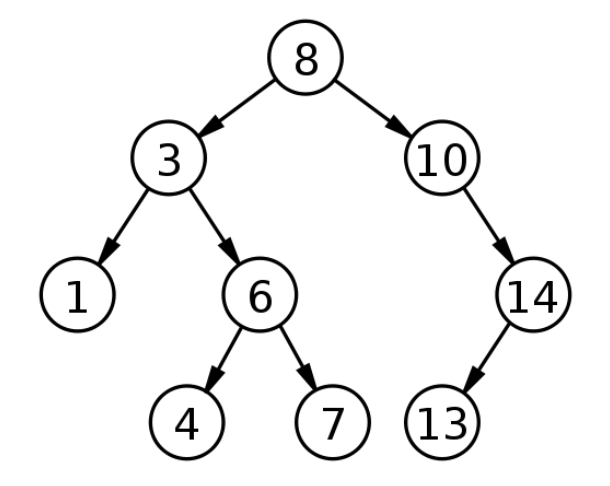
\includegraphics[width=.42\textwidth]{figuras/BST.png}
			\caption{Wikipédia}
		\end{figure}
	\end{center}
\end{block}
\end{frame}

%- - - - - - - - - - - - - - - - - - - - - - - - - - - - - - - - - SLIDE -
\begin{frame}
\frametitle{Estruturas de Dados Básicas}
\begin{block}{Binary Search Tree - O que elas podem fazer}
	\begin{itemize}
		\bitem Suporta três operações
		\begin{itemize}
			\bitem Insere(x): insere um nó com valor x
			\bitem Deleta(x): delete um nó com valor x, se o mesmo existir
			\bitem Encontra(x): retorna o nó com valor x, se o mesmo existir
		\end{itemize}
		\bitem Várias extensões são possíveis
		\begin{itemize}
			\bitem Conte(x): conta o número de nós com valor $\leq$ x
			\bitem PegaProximo(x): retorna o menor nó com valor $\geq$ x
		\end{itemize}
	\end{itemize}
\end{block}
\end{frame}

%- - - - - - - - - - - - - - - - - - - - - - - - - - - - - - - - - SLIDE -
\begin{frame}
\frametitle{Estruturas de Dados Básicas}
\begin{block}{Binary Search Tree - Competições de Programação}
	\begin{itemize}
		\bitem Uma implementação simples não garante a eficiência
		\begin{itemize}
			\bitem No pior caso, a altura da árvore se torna $n$ (o que faz a BST inútil)
			\bitem Garantir complexidade de tempo $O(log\ n)$ por operação requer um balanceamento da árvore (difícil de implementar)
			\bitem Vamos pular os detalhes de implementação
		\end{itemize}
		\bitem Use as implementações prontas da STL!
		\begin{itemize}
			\bitem set, map \textbf{(C++)}
		\end{itemize}
	\end{itemize}
\end{block}
\end{frame}

%- - - - - - - - - - - - - - - - - - - - - - - - - - - - - - - - - SLIDE -
\begin{frame}
\frametitle{Estruturas de Dados Básicas}
\begin{block}{STL - Set}
\begin{itemize}
	\bitem empty() Testa se o set está vazio
	\begin{itemize}
		\bitem Complexidade - $O(1)$
	\end{itemize}
	\bitem size() Retorna o tamanho do set
	\begin{itemize}
		\bitem Complexidade - $O(1)$
	\end{itemize}
	\bitem insert(elemento) Insere um elemento no set
	\begin{itemize}
		\bitem Complexidade - $O(log\ n)$
	\end{itemize}
	\bitem erase(element) Deleta um elemento do set
	\begin{itemize}
		\bitem Complexidade - $O(log\ n)$
	\end{itemize}
	\bitem clear() Limpa o set
	\begin{itemize}
		\bitem Complexidade - $O(n)$
	\end{itemize}
\end{itemize}
\end{block}
\end{frame}

%- - - - - - - - - - - - - - - - - - - - - - - - - - - - - - - - - SLIDE -
\begin{frame}
\frametitle{Estruturas de Dados Básicas}
\begin{block}{STL - Map}
\begin{itemize}
	\bitem empty() Testa se o map está vazio
	\begin{itemize}
		\bitem Complexidade - $O(1)$
	\end{itemize}
	\bitem size() Retorna o tamanho do map
	\begin{itemize}
		\bitem Complexidade - $O(1)$
	\end{itemize}
	\bitem insert(elemento) Insere um elemento no map
	\begin{itemize}
		\bitem Complexidade - $O(log\ n)$
	\end{itemize}
	\bitem erase(element) Deleta um elemento do map
	\begin{itemize}
		\bitem Complexidade - $O(log\ n)$
	\end{itemize}
	\bitem clear() Limpa o set
	\begin{itemize}
		\bitem Complexidade - $O(n)$
	\end{itemize}
\end{itemize}
\end{block}
\end{frame}

%- - - - - - - - - - - - - - - - - - - - - - - - - - - - - - - - - SLIDE -
\begin{frame}
\frametitle{STL - Funções úteis}
\begin{block}{cctype}
\begin{itemize}
	\bitem Funções determinantes de propriedades dos caracteres: isalnum, isalpha, isblank, iscntrl, isdigit, isgraph, islower, isprint, ispunct, isspace, isupper, isxdigit
	\bitem Funções de conversão: tolower, toupper
\end{itemize}
\end{block}
\end{frame}

%- - - - - - - - - - - - - - - - - - - - - - - - - - - - - - - - - SLIDE -
\begin{frame}
\frametitle{STL - Funções úteis}
\begin{block}{algorithm}
\begin{itemize}
	\bitem swap, unique, reverse, sort, lower\_bound, upper\_bound, binary\_search, set\_intersection, min, max, min\_element, max\_element, next\_permutation, prev\_permutation ...
\end{itemize}
\end{block}
\end{frame}

%- - - - - - - - - - - - - - - - - - - - - - - - - - - - - - - - - SLIDE -
\begin{frame}
\frametitle{STL - Funções úteis}
\begin{block}{cmath}
\begin{itemize}
	\bitem cos, sin, tan, acos, asin, atan, atan2, log, log10, sqrt, ceil, floor...
\end{itemize}
\end{block}
\end{frame}

%- - - - - - - - - - - - - - - - - - - - - - - - - - - - - - - - - SLIDE -
\begin{frame}
\frametitle{Leituras Recomendadas}

\begin{block}{}
\begin{itemize}
\tiny
	\bitem \url{http://community.topcoder.com/tc?module=Static&d1=tutorials&d2=complexity1}
	\bitem \url{http://community.topcoder.com/tc?module=Static&d1=tutorials&d2=complexity2}
	\bitem \url{http://www.inf.ufg.br/~cc080153/tap/material/stl_part1.pdf}
	\bitem \url{http://www.inf.ufg.br/~cc080153/tap/material/stl_part2.pdf}
	\bitem \url{http://www.inf.ufg.br/~cc080153/tap/material/stl_part3.pdf}	
	\bitem \url{http://community.topcoder.com/tc?module=Static&d1=tutorials&d2=dataStructures}
%	\bitem \url{http://community.topcoder.com/tc?module=Static&d1=tutorials&d2=bitManipulation}
	\bitem \url{http://community.topcoder.com/tc?module=Static&d1=tutorials&d2=standardTemplateLibrary}
	\bitem \url{http://community.topcoder.com/tc?module=Static&d1=tutorials&d2=standardTemplateLibrary2}
\end{itemize}
\end{block}

\end{frame}

%%- - - - - - - - - - - - - - - - - - - - - - - - - - - - - - - - - ESTRUTURAS DE DADOS -
%%- - - - - - - - - - - - - - - - - - - - - - - - - - - - - - - - - SLIDE -
%
%% array static / vector ..
%% problema / motivação
%%    recuperar um valor de acordo com diferentes politicas
%% 	 stack
%% 	 queue
%% 	 PQ
%% C++ String
%% BST -- set, map
%% STL - sort, algorithm...
%
%
%\begin{frame}
%\frametitle{Estruturas de Dados Básicas}
%\begin{block}{Objetivo}
%Apresentar algumas estruturas de dados básicas e comumente usadas em competições.
%\begin{itemize}
%	\bitem Foco na aplicação das mesmas, utilizando a \emph{Standard Library} do C++.
%\end{itemize}
%\end{block}
%\end{frame}
%
%%- - - - - - - - - - - - - - - - - - - - - - - - - - - - - - - - - SLIDE -
%\begin{frame}
%\frametitle{Estruturas de Dados Básicas}
%\begin{block}{Vetores}
%\begin{itemize}
%	\bitem Vetor estático -- \texttt{int array[256];}
%	\bitem Vetor dinâmico 
%	\begin{itemize}
%		\bitem C++ \emph{Standard Library} \textbf{vector}, Java \textbf{Vector}
%	\end{itemize}
%\end{itemize}
%\end{block}
%
%\begin{block}{STL vector}
%\begin{itemize}
%	\item[] \texttt{\#include<vector>}
%	\begin{itemize}
%		\item[] \texttt{vector<int> a;    a.push\_back(x); }
%		\item[] \texttt{vector<int> a(15);  a[10] = 42;}
%		\item[] \texttt{vector<int> a(15, -1);}
%		\item[] \texttt{vector<char> b; vector<double> c;}
%		\item[] \texttt{vector<int> a; a.resize(1337); }
%	\end{itemize}
%\end{itemize}
%\end{block}
%\end{frame}
%
%%- - - - - - - - - - - - - - - - - - - - - - - - - - - - - - - - - SLIDE -
%\defverbatim[colored]\lstI{
%\begin{lstlisting}[language=C++]
%void semestre() {
%	while(true) { /* nunca para */
%		tarefa x = PegaNovaTarefa(tarefas);
%		processa(x);
%		/* novas tarefas podem surgir */
%	}
%}
%\end{lstlisting}
%}
%
%\begin{frame}
%\frametitle{Estruturas de Dados Básicas}
%\begin{block}{Semestre típico}
%\lstI
%\end{block}
%
%\begin{block}{}
%	\begin{itemize}
%		\item PegaNovaTarefa() decide a ordem em que as tarefas serão selecionadas.
%	\end{itemize}
%\end{block}
%
%\end{frame}
%
%%- - - - - - - - - - - - - - - - - - - - - - - - - - - - - - - - - SLIDE -
%\begin{frame}
%\frametitle{Estruturas de Dados Básicas}
%\begin{block}{PegaNovaTarefa()}
%\begin{itemize}
%	\item Possíveis comportamentos de PegaNovaTarefa():
%	\begin{itemize}
%		\item Retorna a tarefa mais nova
%		\item Retorna a tarefa mais velha
%		\item Retorna a tarefa mais urgente
%		\item Retorna a tarefa mais fácil
%	\end{itemize}
%	\item Queremos que PegaNovaTarefa() execute no menor tempo possível:
%	\begin{itemize}
%		\item ... organizando as tarefas de uma forma inteligente
%	\end{itemize}
%\end{itemize}
%\end{block}
%\end{frame}
%
%%- - - - - - - - - - - - - - - - - - - - - - - - - - - - - - - - - SLIDE -
%\begin{frame}
%\frametitle{Estruturas de Dados Básicas}
%\begin{block}{PegaNovaTarefa()}
%\begin{itemize}
%	\item Possíveis comportamentos de PegaNovaTarefa():
%	\begin{itemize}
%		\item Retorna a tarefa mais nova (pilha)
%		\item Retorna a tarefa mais velha
%		\item Retorna a tarefa mais urgente
%		\item Retorna a tarefa mais fácil
%	\end{itemize}
%	\item Queremos que PegaNovaTarefa() execute no menor tempo possível:
%	\begin{itemize}
%		\item ... organizando as tarefas de uma forma inteligente
%	\end{itemize}
%\end{itemize}
%\end{block}
%\end{frame}
%
%%- - - - - - - - - - - - - - - - - - - - - - - - - - - - - - - - - SLIDE -
%\begin{frame}
%\frametitle{Estruturas de Dados Básicas}
%\begin{block}{Pilha}
%\begin{itemize}
%	\item Ultimo que entra é o primeiro que sai (LIFO)
%	\item Suporta três operações de tempo constante:
%	\begin{itemize}
%		\item Push(x): Insere x na pilha
%		\item Pop(): Remove o item mais novo
%		\item Top(): Retorna o item mais novo
%	\end{itemize}
%	\item Implementação pronta na STL (stack)
%\end{itemize}
%\end{block}
%\end{frame}
%
%%- - - - - - - - - - - - - - - - - - - - - - - - - - - - - - - - - SLIDE -
%\begin{frame}
%\frametitle{Estruturas de Dados Básicas}
%Falar mais da pilha da STL...
%\end{frame}
%
%%- - - - - - - - - - - - - - - - - - - - - - - - - - - - - - - - - SLIDE -
%\begin{frame}
%\frametitle{Estruturas de Dados Básicas}
%\begin{block}{PegaNovaTarefa()}
%\begin{itemize}
%	\item Possíveis comportamentos de PegaNovaTarefa():
%	\begin{itemize}
%		\item Retorna a tarefa mais nova (pilha)
%		\item Retorna a tarefa mais velha
%		\item Retorna a tarefa mais urgente
%		\item Retorna a tarefa mais fácil
%	\end{itemize}
%	\item Queremos que PegaNovaTarefa() execute no menor tempo possível:
%	\begin{itemize}
%		\item ... organizando as tarefas de uma forma inteligente
%	\end{itemize}
%\end{itemize}
%\end{block}
%\end{frame}
%
%%- - - - - - - - - - - - - - - - - - - - - - - - - - - - - - - - - SLIDE -
%\begin{frame}
%\frametitle{Estruturas de Dados Básicas}
%\begin{block}{PegaNovaTarefa()}
%\begin{itemize}
%	\item Possíveis comportamentos de PegaNovaTarefa():
%	\begin{itemize}
%		\item Retorna a tarefa mais nova (pilha)
%		\item Retorna a tarefa mais velha (fila)
%		\item Retorna a tarefa mais urgente
%		\item Retorna a tarefa mais fácil
%	\end{itemize}
%	\item Queremos que PegaNovaTarefa() execute no menor tempo possível:
%	\begin{itemize}
%		\item ... organizando as tarefas de uma forma inteligente
%	\end{itemize}
%\end{itemize}
%\end{block}
%\end{frame}
%
%%- - - - - - - - - - - - - - - - - - - - - - - - - - - - - - - - - SLIDE -
%\begin{frame}
%\frametitle{Estruturas de Dados Básicas}
%\begin{block}{Fila}
%\begin{itemize}
%	\item Primeiro que entra é o primeiro que sai (FIFO)
%	\item Suporta três operações de tempo constante:
%	\begin{itemize}
%		\item Push(x): Insere x na fila
%		\item Pop(): Remove o item mais velho
%		\item Front(): Retorna o item mais velho
%	\end{itemize}
%	\item Implementação pronta na STL (queue)
%\end{itemize}
%\end{block}
%\end{frame}
%
%%- - - - - - - - - - - - - - - - - - - - - - - - - - - - - - - - - SLIDE -
%\begin{frame}
%\frametitle{Estruturas de Dados Básicas}
%Falar mais da fila da STL...
%\end{frame}
%
%%- - - - - - - - - - - - - - - - - - - - - - - - - - - - - - - - - SLIDE -
%\begin{frame}
%\frametitle{Estruturas de Dados Básicas}
%\begin{block}{PegaNovaTarefa()}
%\begin{itemize}
%	\item Possíveis comportamentos de PegaNovaTarefa():
%	\begin{itemize}
%		\item Retorna a tarefa mais nova (pilha)
%		\item Retorna a tarefa mais velha (fila)
%		\item Retorna a tarefa mais urgente
%		\item Retorna a tarefa mais fácil
%	\end{itemize}
%	\item Queremos que PegaNovaTarefa() execute no menor tempo possível:
%	\begin{itemize}
%		\item ... organizando as tarefas de uma forma inteligente
%	\end{itemize}
%\end{itemize}
%\end{block}
%\end{frame}
%
%%- - - - - - - - - - - - - - - - - - - - - - - - - - - - - - - - - SLIDE -
%\begin{frame}
%\frametitle{Estruturas de Dados Básicas}
%\begin{block}{PegaNovaTarefa()}
%\begin{itemize}
%	\item Possíveis comportamentos de PegaNovaTarefa():
%	\begin{itemize}
%		\item Retorna a tarefa mais nova (pilha)
%		\item Retorna a tarefa mais velha (fila)
%		\item Retorna a tarefa mais urgente (fila de prioridades)
%		\item Retorna a tarefa mais fácil
%	\end{itemize}
%	\item Queremos que PegaNovaTarefa() execute no menor tempo possível:
%	\begin{itemize}
%		\item ... organizando as tarefas de uma forma inteligente
%	\end{itemize}
%\end{itemize}
%\end{block}
%\end{frame}
%
%%- - - - - - - - - - - - - - - - - - - - - - - - - - - - - - - - - SLIDE -
%\begin{frame}
%\frametitle{Estruturas de Dados Básicas}
%\begin{block}{PegaNovaTarefa()}
%\begin{itemize}
%	\item Possíveis comportamentos de PegaNovaTarefa():
%	\begin{itemize}
%		\item Retorna a tarefa mais nova (pilha)
%		\item Retorna a tarefa mais velha (fila)
%		\item Retorna a tarefa mais urgente (fila de prioridades)
%		\item Retorna a tarefa mais fácil (fila de prioridades)
%	\end{itemize}
%	\item Queremos que PegaNovaTarefa() execute no menor tempo possível:
%	\begin{itemize}
%		\item ... organizando as tarefas de uma forma inteligente
%	\end{itemize}
%\end{itemize}
%\end{block}
%\end{frame}
%
%%- - - - - - - - - - - - - - - - - - - - - - - - - - - - - - - - - SLIDE -
%\begin{frame}
%\frametitle{Estruturas de Dados Básicas}
%\begin{block}{Fila de prioridades}
%\begin{itemize}
%	\item Cada elemento em uma fila de prioridades tem um valor que corresponde a sua prioridade
%	\item Suporta três operações
%	\begin{itemize}
%		\item Push(x, p): Insere x com prioridade p na fila de prioridades
%		\item Pop(): Remove o elemento com a maior prioridade
%		\item Top(): Retorna o elemento com a maior prioridade
%	\end{itemize}
%	\item Todas as operações podem ser feitas de forma rápida se implementadas usando uma Heap
%	\item Implementação com Heap pronta na STL (priority\_queue)
%\end{itemize}
%\end{block}
%\end{frame}
%
%%- - - - - - - - - - - - - - - - - - - - - - - - - - - - - - - - - SLIDE -
%\begin{frame}
%\frametitle{Estruturas de Dados Básicas}
%Falar mais da fila de prioridades da STL...
%\end{frame}
%
%%- - - - - - - - - - - - - - - - - - - - - - - - - - - - - - - - - SLIDE -
%\begin{frame}
%\frametitle{Estruturas de Dados Básicas}
%Falar de BST...
%\end{frame}
%
%%- - - - - - - - - - - - - - - - - - - - - - - - - - - - - - - - - SLIDE -
%\begin{frame}
%\frametitle{Estruturas de Dados Básicas}
%Falar de Heap...
%\end{frame}
%
%%- - - - - - - - - - - - - - - - - - - - - - - - - - - - - - - - - SLIDE -
%\begin{frame}
%\frametitle{Estruturas de Dados Básicas}
%Falar de Set da STL...
%\end{frame}
%
%%- - - - - - - - - - - - - - - - - - - - - - - - - - - - - - - - - SLIDE -
%\begin{frame}
%\frametitle{Estruturas de Dados Básicas}
%Falar de Map da STL...
%\end{frame}
%
%%- - - - - - - - - - - - - - - - - - - - - - - - - - - - - - - - - SLIDE -
%\begin{frame}
%\frametitle{Estruturas de Dados Básicas}
%Falar de coisas comum da algorithm e stdlib (stdlib: abs; cctype: tudo; algoritm: swap, unique, reverse, random\_shuffle(?), sort, lower\_bound, upper\_bound, binary\_search, set\_* (?), min, max, min\_element, max\_element, next\_permutation, prev\_permutation
%\end{frame}
%
%%- - - - - - - - - - - - - - - - - - - - - - - - - - - - - - - - - SLIDE -
%\begin{frame}
%\frametitle{Leituras Recomendadas}
%
%\begin{block}{}
%\begin{itemize}
%\tiny
%	\bitem \url{http://community.topcoder.com/tc?module=Static&d1=tutorials&d2=complexity1}
%	\bitem \url{http://community.topcoder.com/tc?module=Static&d1=tutorials&d2=complexity2}
%	\bitem \url{http://www.inf.ufg.br/~cc080153/tap/material/stl_part1.pdf}
%	\bitem \url{http://www.inf.ufg.br/~cc080153/tap/material/stl_part2.pdf}
%	\bitem \url{http://www.inf.ufg.br/~cc080153/tap/material/stl_part3.pdf}	
%	\bitem \url{http://community.topcoder.com/tc?module=Static&d1=tutorials&d2=dataStructures}
%%	\bitem \url{http://community.topcoder.com/tc?module=Static&d1=tutorials&d2=bitManipulation}
%	\bitem \url{http://community.topcoder.com/tc?module=Static&d1=tutorials&d2=standardTemplateLibrary}
%	\bitem \url{http://community.topcoder.com/tc?module=Static&d1=tutorials&d2=standardTemplateLibrary2}
%\end{itemize}
%\end{block}
%
%\end{frame}